% RAG and retrieval benchmarking on SciFact (companion to report.md)
% Figures: from this repo, compile inside latex/ with pdflatex; paths point up one level.
% On Overleaf, if you upload both this .tex and report_assets to the project root,
% replace the graphicspath line below with: \graphicspath{{report_assets/}}
\documentclass[11pt,a4paper]{article}
\usepackage[margin=1in]{geometry}
\usepackage{graphicx}
\usepackage{booktabs}
\usepackage{hyperref}
\usepackage{amsmath}
\usepackage{caption}

\graphicspath{{../report_assets/}}

\title{RAG Comparison Benchmarking on SciFact\\
\large Dense, sparse, and hybrid retrieval with BEIR evaluation}
\author{R2L Lab onboarding exercise (repository artifact)}
\date{\today}

\begin{document}
\maketitle

\begin{abstract}
This note documents a retrieval only benchmark on the SciFact test split using BEIR style data loading and evaluation. We compare BM25 sparse retrieval, dense retrieval with a MiniLM sentence encoder and FAISS inner product search, linear score fusion hybrids with several alpha weights, and reciprocal rank fusion variants. The best observed configuration in the committed artifacts uses linear hybrid fusion with alpha equal to $0.3$, favoring the dense channel, and achieves the highest NDCG@10 among all recorded runs. The companion Markdown report in the repository adds animated figures and a wider discussion of limitations.
\end{abstract}

\section{Introduction and scope}

The repository supports an R2L Lab style onboarding quiz: implement retrievers, run a standard benchmark, and interpret tradeoffs. The task is \emph{retrieval} in the classical sense. Each system returns a ranked list of documents for each query. There is no generative reader or claim verification model in the pipeline, so metrics measure finding relevant abstracts, not producing final verdicts.

SciFact is appropriate for teaching because queries are short scientific claims and relevance is defined in a fact checking oriented way. That stresses both lexical overlap and semantic similarity.

\section{Technical approach}

\subsection{Corpus preparation}

For every document the code concatenates title and main text into a single string. BM25 uses lowercased whitespace tokenization. Dense retrieval encodes the same raw string with a SentenceTransformer model.

\subsection{Dense retrieval}

The encoder is \texttt{all-MiniLM-L6-v2}. Embeddings are L2 normalized and indexed with FAISS \texttt{IndexFlatIP}, so inner product search corresponds to cosine similarity ranking. Retrieval depth is 100 documents per query.

\subsection{Sparse retrieval}

BM25Okapi indexes tokenized documents. Retrieval depth matches the dense path at 100.

\subsection{Linear hybrid fusion}

For each query, BM25 scores and dense scores are min max normalized separately, then combined as
\begin{equation}
s_{\mathrm{hybrid}}(d) = \alpha\, \hat{s}_{\mathrm{BM25}}(d) + (1-\alpha)\, \hat{s}_{\mathrm{dense}}(d).
\end{equation}
The repository includes runs for $\alpha \in \{0.3, 0.5, 0.7\}$.

\subsection{Reciprocal rank fusion}

RRF merges ranked lists using
\begin{equation}
\mathrm{RRF}(d) = \sum_{\ell \in \{\mathrm{BM25},\mathrm{dense}\}} \frac{1}{k + \mathrm{rank}_\ell(d)}.
\end{equation}
Committed runs use $k \in \{10, 60, 100\}$.

\subsection{Evaluation}

\texttt{evaluation.py} calls BEIR \texttt{EvaluateRetrieval} with cutoffs 10 and 100 for NDCG, MAP, recall, and precision.

\section{Results}

Table~\ref{tab:main} summarizes metrics recomputed from the JSON result files shipped in the repository. The hybrid model with $\alpha = 0.3$ achieves the best NDCG@10.

\begin{table}[htbp]
\centering
\caption{SciFact test split metrics. BM25 row matches sparse results file.}
\label{tab:main}
\begin{tabular}{lcccc}
\toprule
\textbf{Configuration} & \textbf{NDCG@10} & \textbf{NDCG@100} & \textbf{Recall@100} & \textbf{MAP@10} \\
\midrule
BM25 sparse & 0.5597 & 0.5839 & 0.7929 & 0.5147 \\
Dense MiniLM + FAISS & 0.6451 & 0.6767 & 0.9250 & 0.5959 \\
Hybrid $\alpha=0.3$ & \textbf{0.6822} & \textbf{0.7118} & \textbf{0.9367} & \textbf{0.6395} \\
Hybrid $\alpha=0.5$ & 0.6751 & 0.7016 & 0.9300 & 0.6282 \\
Hybrid $\alpha=0.7$ & 0.6244 & 0.6639 & 0.9253 & 0.5824 \\
RRF $k=10$ & 0.6592 & 0.6874 & 0.9287 & 0.6084 \\
RRF $k=60$ & 0.6391 & 0.6752 & 0.9287 & 0.5944 \\
RRF $k=100$ & 0.6335 & 0.6736 & 0.9287 & 0.5919 \\
\bottomrule
\end{tabular}
\end{table}

\section{Figures}

Figure~\ref{fig:ndcg} gives a bar view of NDCG@10. Figure~\ref{fig:scatter} relates recall at 100 to NDCG@10. Animated sweeps that illustrate the hybrid alpha story live in the Markdown report as GIF files, since PDF engines vary in animated image support.

\begin{figure}[htbp]
\centering
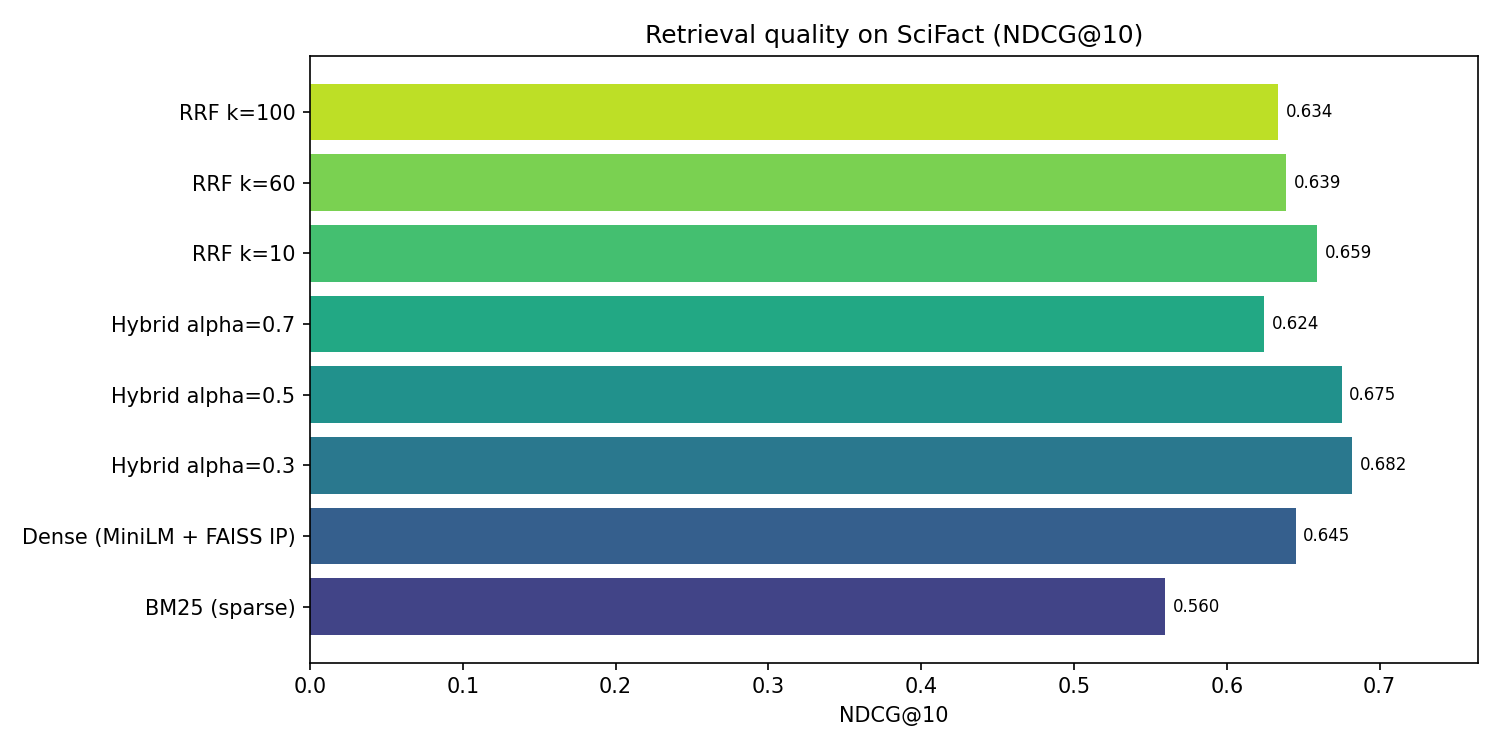
\includegraphics[width=0.95\linewidth]{ndcg10_comparison.png}
\caption{NDCG@10 across all committed runs.}
\label{fig:ndcg}
\end{figure}

\begin{figure}[htbp]
\centering
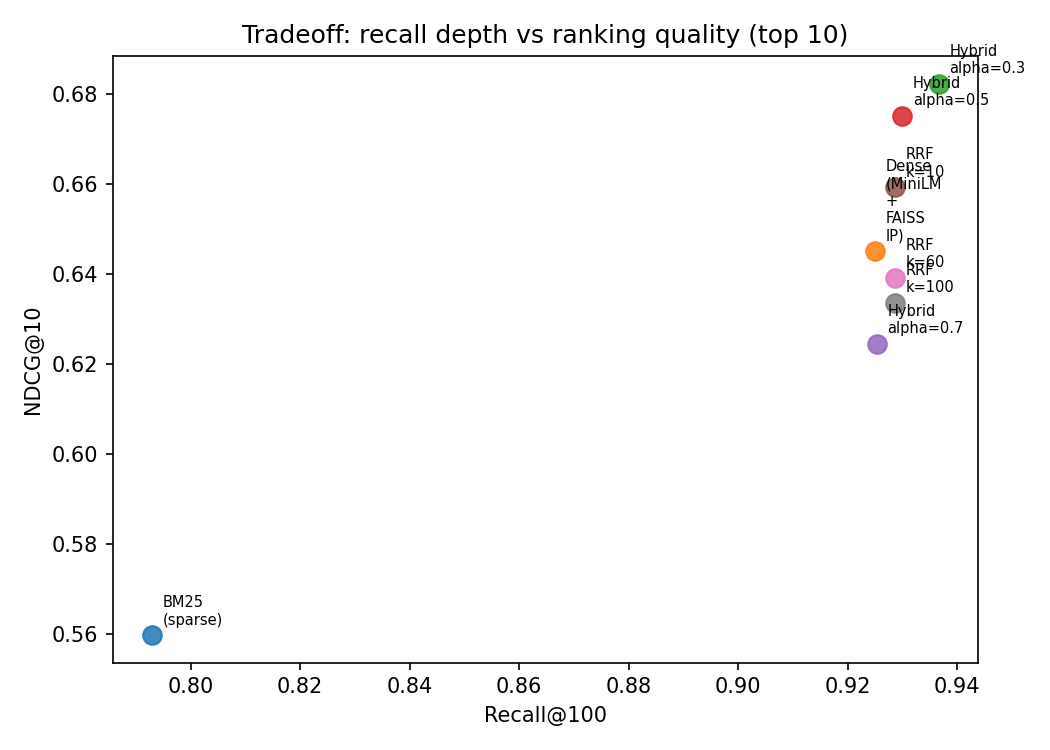
\includegraphics[width=0.78\linewidth]{recall_vs_ndcg10.png}
\caption{Recall@100 versus NDCG@10 with per method labels.}
\label{fig:scatter}
\end{figure}

\section{Discussion}

Dense retrieval alone already improves NDCG@10 substantially over BM25, which matches the expectation that claim wording often diverges from evidence wording. Adding a modest BM25 weight at $\alpha = 0.3$ preserves dense dominance while injecting sparse signal for rare strings. Pushing $\alpha$ to $0.7$ hurts ranking quality here, which suggests sparse scores were noisy relative to the dense channel for this encoder and preprocessing.

RRF with $k=10$ is the strongest RRF setting in the table, yet it remains below the best linear hybrid on NDCG@10. One plausible reason is that min max normalized fusion still uses score magnitudes in a helpful way when both retrievers are already strong.

Several systems cluster near $0.93$ recall at 100, so differences in practical deployments may hinge more on top ten behavior than on deep recall alone.

\section{Limitations and future work}

The study uses a single general purpose embedding model, simple tokenization, and an exact flat FAISS index. None of these choices is tuned for biomedical morphology or large scale corpora. There is no statistical testing on metric differences. The natural next engineering step for higher NDCG@10 is cross encoder reranking on a short candidate list.

\section{Reproducibility}

Clone the repository, install Python dependencies from the \texttt{requirements} file, ensure SciFact sits under \texttt{datasets/scifact/}, rerun retrievers as needed, then run \texttt{evaluation.py} with the path to each results JSON. Figures can be rebuilt with \texttt{python scripts/generate\_report\_figures.py} after installing matplotlib and Pillow.

\vspace{1em}
\noindent\textbf{Repository pointers:} \texttt{report.md} for the full narrative with animated plots; this \texttt{.tex} file for a formal PDF article layout.

\end{document}
